\documentclass{article}

\usepackage{listings}
\usepackage{enumitem}
\usepackage{amsmath}
\usepackage{svg}
\usepackage{hyperref}
\hypersetup{
    colorlinks=true,
    linkcolor=blue,
    filecolor=magenta,      
    urlcolor=cyan,
    pdftitle={Overleaf Example},
    pdfpagemode=FullScreen,
    }

\title{CA Lab: Lab 3}
\author{student: Dimitri Tabatadze}

\begin{document}
    \maketitle

    \section*{Task Description}

    Full adder has 3 inputs and 2 outputs. 
    
    \begin{enumerate}[label={\alph*}]
        \item {Create truth table of full adder. (10 points)}
        \item {Write Boolean expressions for the outputs. (15 points)}
        \item {Draw the circuit diagram for full adder. (10 points)}
        \item {Write the code of adder in Verilog. (50 points)}
    \end{enumerate}

    \section*{Solution}
    
    \begin{enumerate}[label={\alph*)}]
        \item \begin{displaymath}
            \begin{array}{|c c c | c c|}
                A & B & C_{in} & S & C_{out} \\
                \hline
                0 & 0 & 0 & 0 & 0 \\
                0 & 0 & 1 & 1 & 0 \\
                0 & 1 & 0 & 1 & 0 \\
                0 & 1 & 1 & 0 & 1 \\
                1 & 0 & 0 & 1 & 0 \\
                1 & 0 & 1 & 0 & 1 \\
                1 & 1 & 0 & 0 & 1 \\
                1 & 1 & 1 & 1 & 1 \\
            \end{array}
        \end{displaymath}
        \item \begin{displaymath}
            \begin{aligned}
                S
                &= (\overline{A} \land \overline{B} \land C_in) \lor (\overline{A} \land B \land \overline{C_in}) \lor (A \land \overline{B} \land \overline{C_in}) \lor (A \land B \land C_in) \\ 
                &= (\overline{A} \land (\overline{B} \land C_in \lor B \land \overline{C_in})) \lor (A \land (\overline{B} \land \overline{C_in} \lor B \land C_in)) \\
                &= (\overline{A} \land (B \oplus C_in)) \lor (A \land \overline{(B \oplus C_in)}) \\
                &= A \oplus (B \oplus C_in) \\
                &= A \oplus B \oplus C_in
            \end{aligned}
        \end{displaymath}
        \begin{displaymath}
            \begin{aligned}
                C_{out} 
                &= (\overline{A} \land B \land C_{in}) \lor (A \land \overline{B} \land C_{in}) \lor (A \land B \land \overline{C_{in}}) \lor (A \land B \land C_{in}) \\ 
                &= (A \land (\overline{B} \land C_{in} \lor B \land \overline{C_{in}} \lor B \land C_{in})) \lor (\overline{A} \land B \land C_{in}) \\
                &= (A \land (B \lor C_{in})) \lor (\overline{A} \land (B \land C_{in})) \\
                &= (B \land C_{in}) \lor (A \land (B \lor C_{in})) \\
                &= (B \land C_{in}) \lor (A \land B) \lor (A \land C_{in})
            \end{aligned}
        \end{displaymath}
        \item The circuit diagram: 
        \begin{figure}[h]
            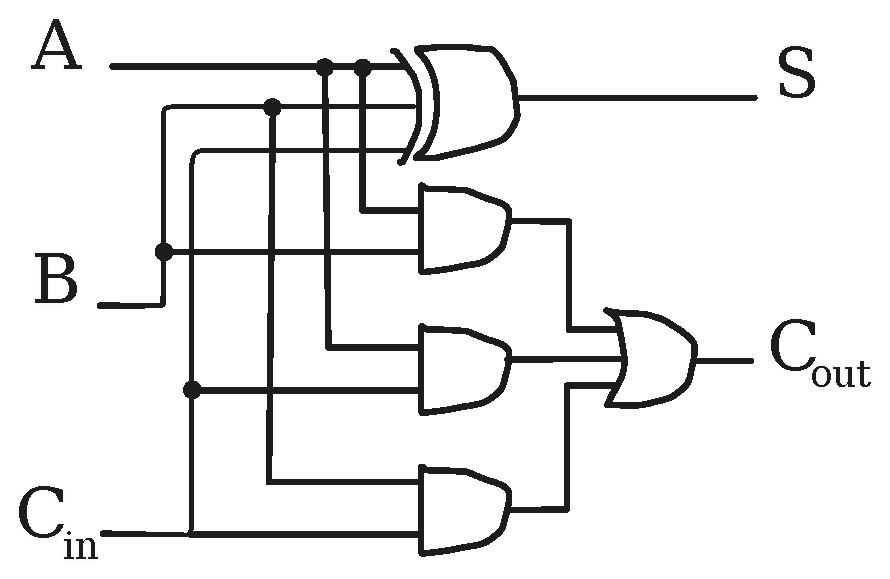
\includegraphics[width=10cm]{full-adder-diagram.eps}
        \end{figure}
        \newpage
        \item The code in Verilog:
        \begin{lstlisting}
module full_adder (
    A,
    B,
    C_in,
    S,
    C_out
);
    input A;
    input B;
    input C_in;

    output S;
    output C_out;

    wire D;
    wire E;
    wire F;

    // Sum
    assign S = A ^ B ^ C_in;
    
    // Carry
    assign D = B & C_in;
    assign E = A & B;
    assign F = A & C_in;
    assign C_out = D | E | F;

endmodule
        \end{lstlisting}
        and a screenshot of highlighted code:
        \newpage
        \begin{figure}[h]
            \includegraphics[width=9cm]{code-screenshot.png}
        \end{figure}
    \end{enumerate}

    \newpage

    \section*{Simulation \& Verification}

    here's the results of the simulation I ran.

    \begin{figure}[h]
        \includegraphics[width=12cm]{screenshot-of-testing.png}
    \end{figure}

    \section*{Conclusion}

    I had to do write verilog in VSCode, I hope it's written the way it was supposed to be.

    \section*{Reference}

    I used \url{https://tldraw.com} for drawing the diagram.

\end{document}